\section{整体设计}
\subsection{模块划分} 
% 或者叫 “整体框架” 之类的?
整体结构图如下。

\begin{figure}[H]
    \centering
    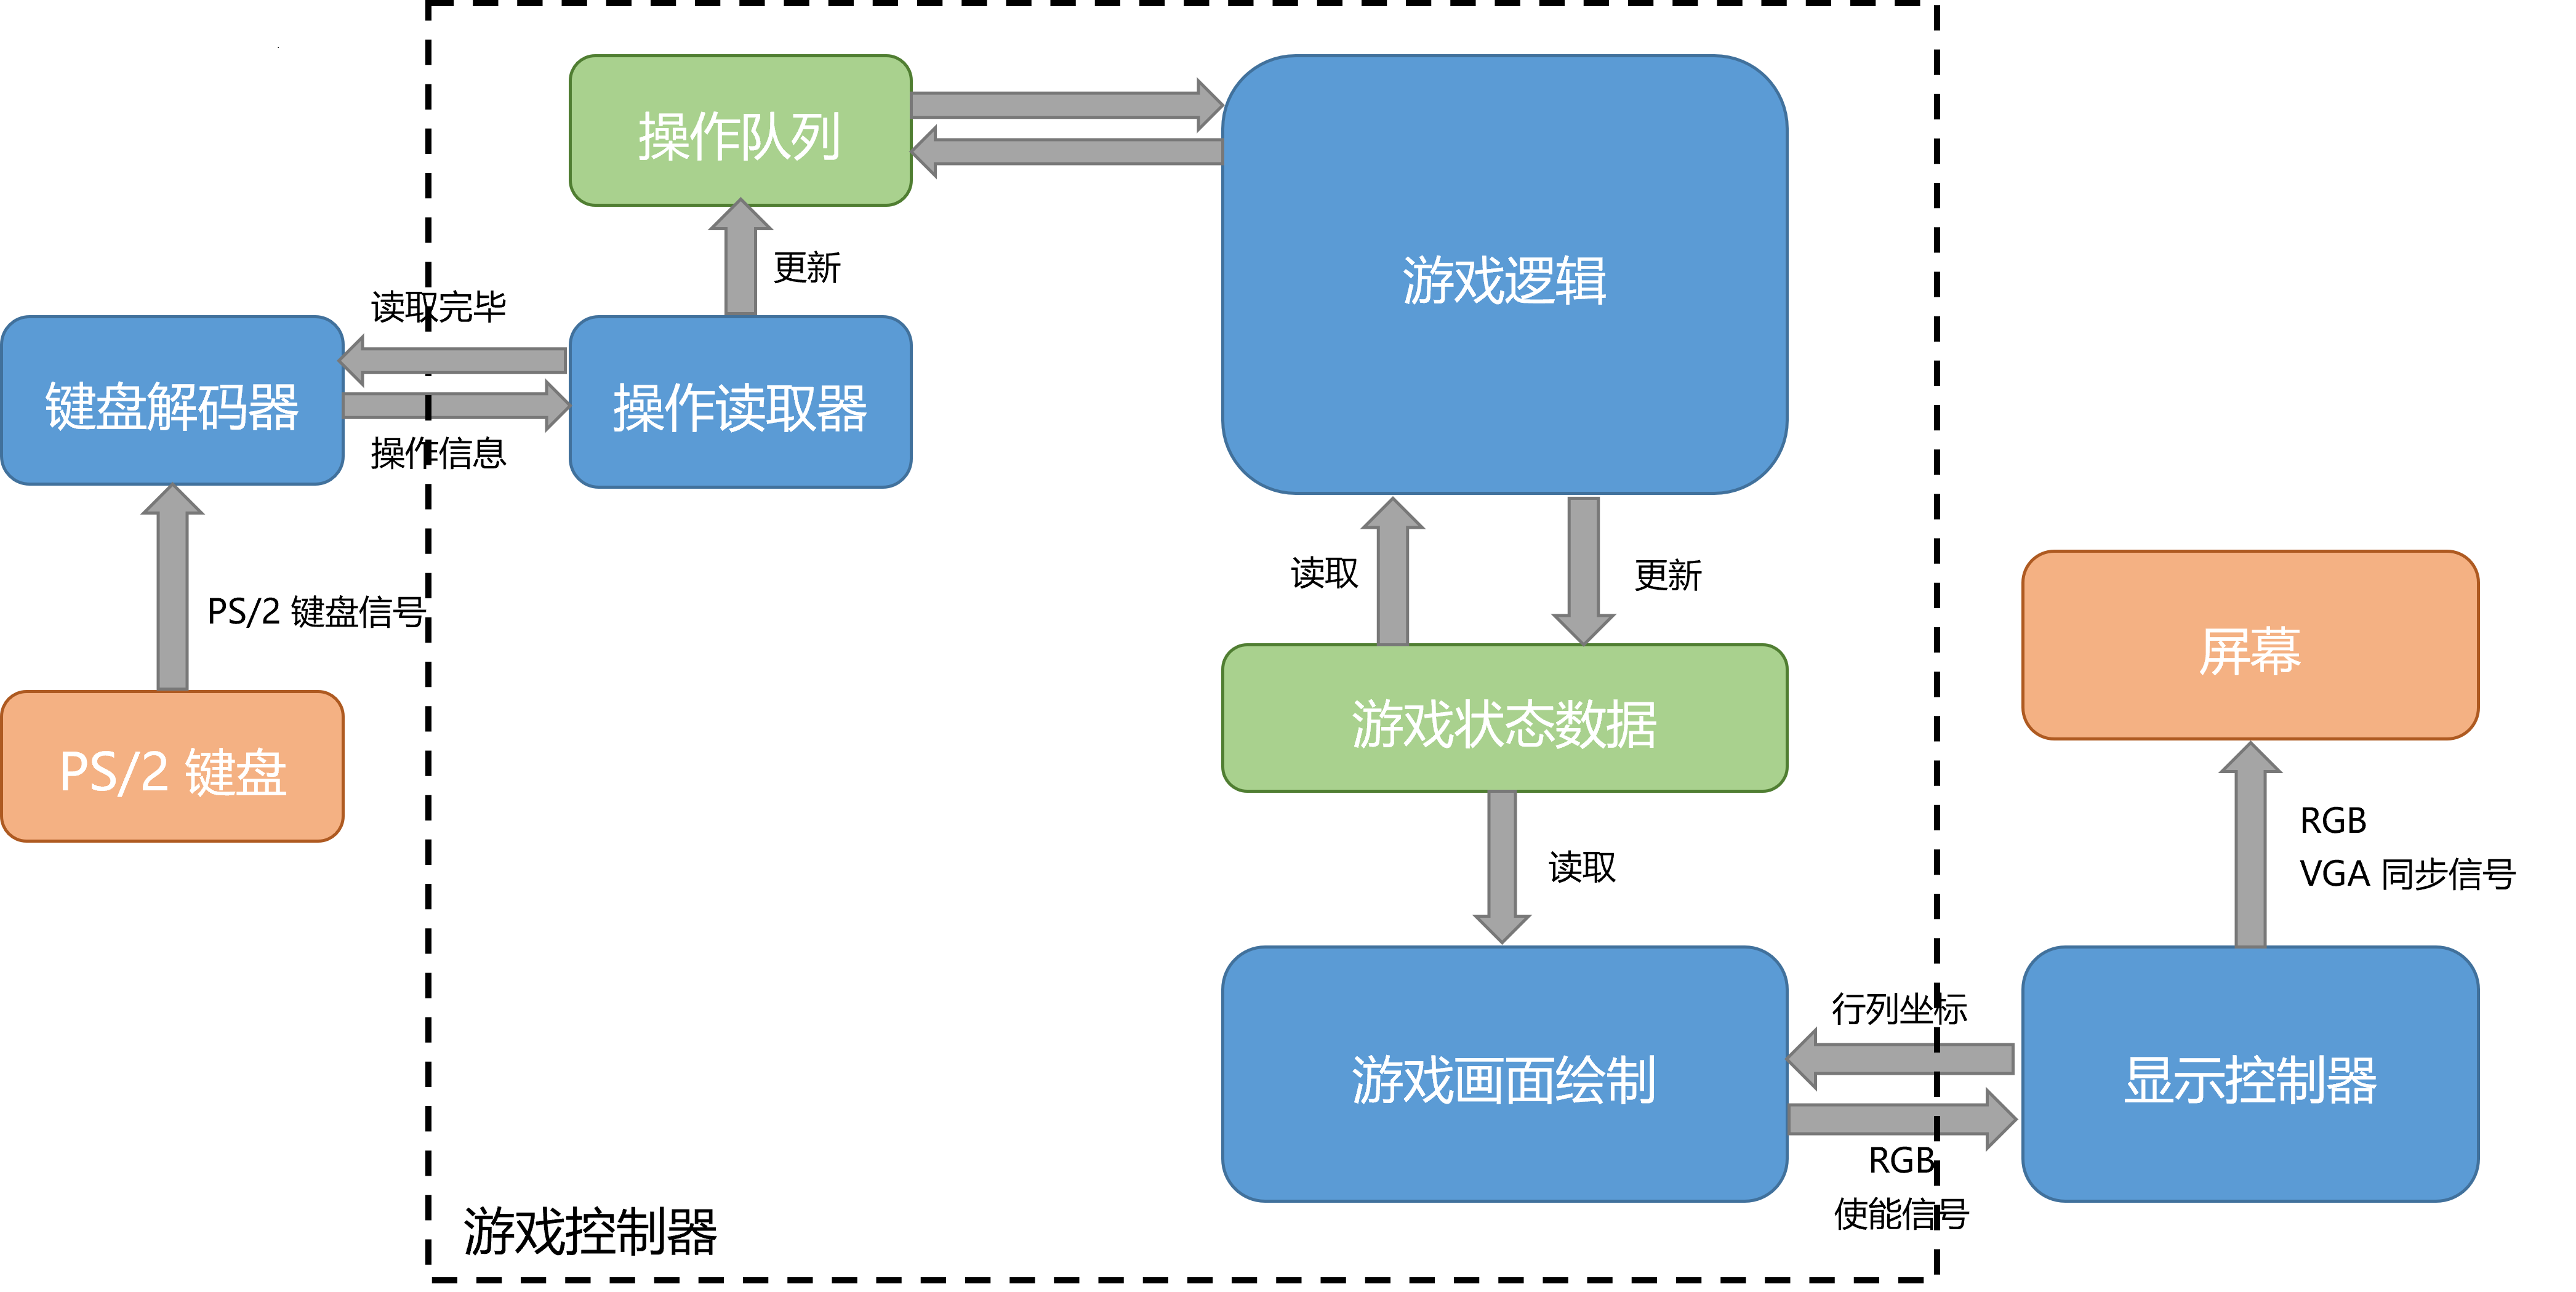
\includegraphics[scale=0.22]{images/structure.png}
    \caption{模块划分}
    \label{fig:structure}
\end{figure}

以上模块图中,橙色框表示外部设备,包括键盘,用以读取玩家的操作;VGA 显示器,用以输出游戏画面。蓝色框表示游戏中的计算和控制模块,包括和外部设备进行交互的键盘解码器和显示控制器,以及处理游戏内部逻辑的其它各模块(整体称为“游戏控制器”)。绿色框表示游戏内部维护的信息。

% 简要介绍各个模块的功能
\textbf{键盘解码器}使用一个状态机,接收并处理PS/2键盘发送的信号(断码),并将对应的操作信息传递给下游的操作读取器。

\textbf{操作读取器}是游戏控制器的上游部分,它读取来自键盘解码器的键盘操作信息,并将此信息写入操作队列(操作队列由操作读取器和游戏控制器共同维护)。

\textbf{游戏逻辑}是游戏控制器的核心部分。它内部用一个状态机维护游戏当前状态。在游戏即将开始时,它产生随机初始棋局和随机先手玩家。在游戏进行中,它从操作队列的队首读取一次键盘的按下信号,并基于游戏状态数据进行相应的计算;完成计算后,对游戏状态数据进行相应修改。

\textbf{游戏画面绘制}基于游戏状态数据,以及下游的显示控制器传回的VGA行列同步信号,计算当前扫描的像素的RGB值并传递给显示控制器。同时,它还判断该像素应该显示棋局信息还是背景图像信息,并向显示控制器输出此信号(即使能信号)。

\textbf{显示控制器}是下游屏幕输出的控制模块。它产生VGA行列同步信号,并将此信号传递回游戏画面绘制部分,从游戏画面绘制部分得到与当前棋局对应的画面信息后,对棋局画面和背景画面进行数据选择,得到最终画面的RGB值。最后,显示控制器将VGA行列同步信号和最终画面的RGB值输出到屏幕。

\subsection{模块间交互信号}

\subsubsection{键盘解码器与游戏控制器} \label{subsubsection:interact-input-logic}

\textbf{从键盘解码器到游戏控制器}
\begin{itemize}
    \item \texttt{ready}:1 bit。1表示有新数据(识别到键盘断码),0表示暂无新数据
    \item \texttt{data}:3 bit。表示识别到的键(WASD、空格、Z)
\end{itemize}

\textbf{从游戏控制器到键盘解码器}
\begin{itemize}
    \item \texttt{read\_fin}:1 bit。1表示数据已经被读取,否则为 0。
\end{itemize}

\subsubsection{游戏控制器与显示控制器}

\textbf{从游戏控制器到显示控制器} \label{subsubsection:interact-logic-output}
\begin{itemize}
    \item \texttt{gen\_red}, \texttt{gen\_green}, \texttt{gen\_blue}:各 8 bit。表示基于游戏局面计算出的游戏画面信息。
    \item \texttt{use\_gen}:1 bit。表示当前像素是使用游戏逻辑生成的棋局图像(1)还是背景图像(0)
\end{itemize}

\textbf{从显示控制器到游戏控制器}
\begin{itemize}
    \item \texttt{hdata\_o}, \texttt{vdata\_o}:各 10 bit。表示当前扫描到的行列坐标。
\end{itemize}


\subsection{文件结构}
% 需要写出每个文件对应以上模块划分图中的哪些部分(模块)

本项目提交的压缩包中的 \verb|design/| 为实验的完整工程。\textbf{在该目录下}, \texttt{digital-design.sof} 为编译后的 bitstream 二进制文件;\texttt{src/} 目录下为源代码(ip 核除外)。

\texttt{src/} 目录下的文件如下(以下按对应模块的层次关系排列):

\begin{itemize}
    \item \texttt{mod\_top.sv} :项目的顶层文件
    \begin{itemize}
        \item \texttt{Keyboard\_Decoder.sv} :键盘解码器
        \item \texttt{Game\_Controller.sv} :游戏控制器
        \begin{itemize}
            \item \texttt{Counter.sv} :循环计数器,(计数频率较高时)可用于产生小范围内的伪随机数
            \item \texttt{Number\_Choose.sv} :用于显示数码
            \item \texttt{Number\_Transfer.sv} :用于计算一个三位数的百位、十位、个位
            \item \texttt{Random\_Boards\_Library.sv} :初始棋盘库,由 \texttt{random\_boards.py} 生成,用于随机选择初始棋盘
        \end{itemize}
        \item \texttt{Screen\_Controller.sv} :显示控制器
        \begin{itemize}
            \item \texttt{Background\_Painter.sv} :用于绘制背景图像
            \item \texttt{vga.v}: VGA 控制器,用于生成 VGA 行列扫描信号
        \end{itemize}
    \end{itemize}
\end{itemize}


\subsection{分工情况}

分工情况如下:
\begin{itemize}
    \item 总体架构设计:陈鑫圣
    \item 输入部分:周晋、陈鑫圣
    \item 游戏逻辑部分:陈鑫圣
    \item 输出部分:周晋
    \item 报告撰写:陈鑫圣、周晋
\end{itemize}